\documentclass{article}

\usepackage{tikz}
\usetikzlibrary{arrows.meta}

\begin{document}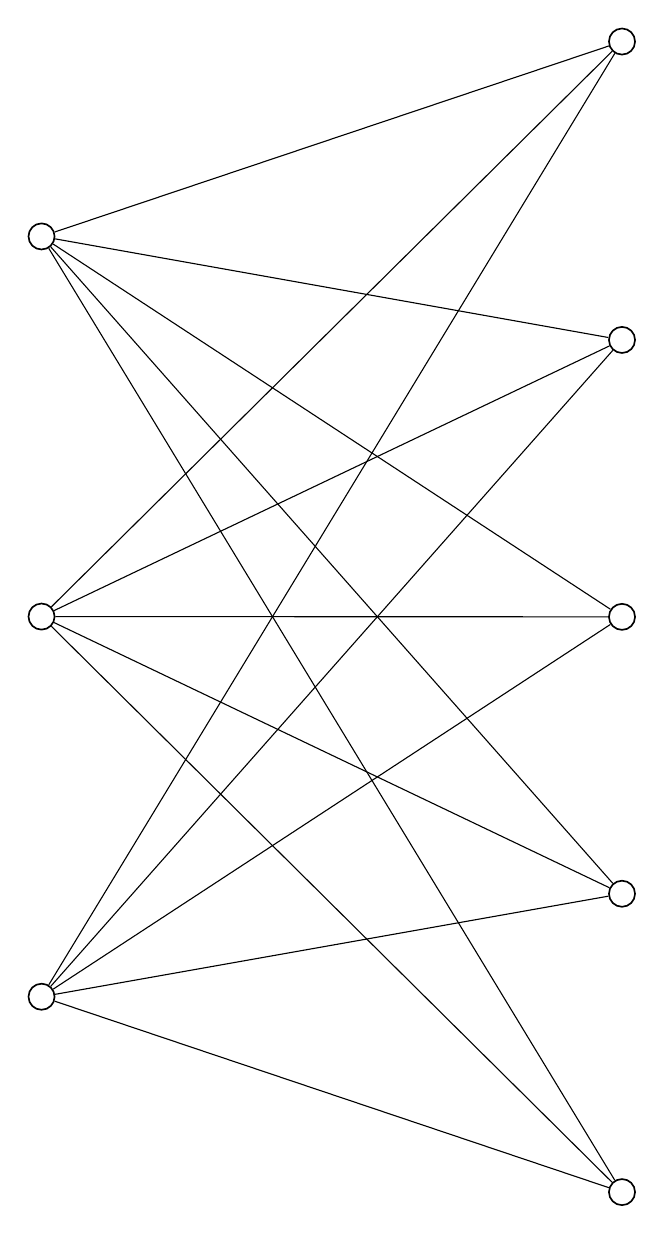
\begin{tikzpicture}[>={Latex},
  default/.style={draw=black, semithick, solid, fill=white, solid, }]
\node[default, circle, ] (A) at (-4.607330134264019, -4.825959979381407) {};
\node[default, circle, ] (B) at (-4.607330134264017, 4.829821971406879) {};
\node[default, circle, ] (C) at (-4.607330134264016, 0.0020797008184051946) {};
\node[default, circle, ] (D) at (2.7644329758871597, -3.5180005328267048) {};
\node[default, circle, ] (E) at (2.7644329758871597, 7.304951073000365) {};
\node[default, circle, ] (F) at (2.7644329758871575, -7.3070692108715365) {};
\node[default, circle, ] (G) at (2.764432975887162, -0.0013683318305802434) {};
\node[default, circle, ] (H) at (2.7644329758871553, 3.515409547207255) {};
\draw [] (A) -- (D);
\draw [] (A) -- (E);
\draw [] (A) -- (F);
\draw [] (A) -- (G);
\draw [] (A) -- (H);
\draw [] (B) -- (D);
\draw [] (B) -- (E);
\draw [] (B) -- (F);
\draw [] (B) -- (G);
\draw [] (B) -- (H);
\draw [] (C) -- (D);
\draw [] (C) -- (E);
\draw [] (C) -- (F);
\draw [] (C) -- (G);
\draw [] (C) -- (H);
\end{tikzpicture}
\end{document}
